\section*{FAQ:}
\begin{enumerate}
  \item 我不太会\LaTeX{}有什么可以参考的资料吗?\,\,\emph{安装和升级详见}《install-latex-guide-zh-cn》,\emph{入门教程}见《Ishort-zh-cn》,\emph{都在群文件},本手册第一章内容是计算机基础知识(已完成)\emph{许多
  常见的问题可以在这里找到}。
  第二章是\LaTeX{}基础知识(待完善),后面是手册的使用说明(待完善)。纸质书籍推荐《LaTeX入门》,《LaTeX范例学习与试卷论文排版》。
  \item 使用哪个\LaTeX{}发行版?\,\,夏学长的新模版使用\TeX{} Live,邓老师的旧模版使用C\TeX{},两个发行版不可以混用,发行版的相关知识见\ref{subsub:fxb}节。C\TeX{}存在一些
        无法解决的问题,因此现在不推荐,详见\ref{subsub:labmwt}节。
  \item 如何检测自己装了哪个版本?\,\,命令行(控制台)运行命令latex,观察弹出来的信息可以知道版本。本群的教程安装的是\TeX{} Live。
  \item 好多资料都提到“运行xx指令”,“命令行/控制台运行xx”都是什么意思?\,\,都是指在命令行下运行指令,相关知识见\ref{subsec:mlh}节。
  \item 新旧模版有什么区别?新模版有什么优势?\,\,在基本的语法指令方面,两个模版基本没有区别。旧模版的存在的问题详见\url{https://gitee.com/xkwxdyy/CCNUthesis}拉到下面有原因说明,
        新模版是为了解决这些问题而进行的重写。
  \item 安装好后桌面怎么没有图标?\,\,请认真阅读\ref{sub:by}节。
  \item 用Texstudio一打开模版就全是乱码,怎么办?\,\,你一定打开了邓老师的旧模板,原因和解决方案详见\ref{bm}节编码的知识。
  
        \emph{补充说明:}Texstudio仅仅是个代码编辑器(详见\ref{sub:by}),能不能正常使用模版与选择的代码编辑器无关,与发行版有关!
  \item 一编译就报一堆错怎么办?\,\,先确认安装的\LaTeX{}发行版和使用的模版是否配套!新模版还需要保证模版是最新的,并且将宏包升级到最新,仍然详见《install-latex-guide-zh-cn》。
  报错信息分成两类,warning(警告)和error(错误),一般情况下只需要在意error。其次,我们应该通过翻译器等方式读懂报错信息,
       并定位错误的代码,检查自己是否有语法错误或者打错,必要时借助搜索引擎或者直接提问,查错的经验需要多多积累。

       \emph{快速排查}:(1)首次编译模版报大量错误,基本上说明发行版和模版不匹配!请检查版本!(2)检查编译方式,新模板为xelatex,旧模版为pdflatex,编译方式的内容见\ref{subsub:yy}节。
       (3)错误\verb"“File ‘ninecolors.sty’ not found. \begin{document}”"的解决办法:如果安装的是TeX Live 2021此错误的原因是没有更新宏包,更新的方法详见群文件《install-latex-guide-zh-cn》1.4节或者在开始菜单找TeX Live Shell来更新。如果安装了版本较旧比如是2020,需要卸载后重新安装,方法仍见《install-latex-guide-zh-cn》第一章。
  \item 遇到了自己无法解决的问题应该怎么办?\,\,到链接\url{https://gitee.com/xkwxdyy/CCNUthesis},选择\emph{issues}菜单,里面有开启中和已完成,
        “已完成”中的问题是有人问过且已经被解决的,应当优先查阅;“开启中”的问题是尚未解决的。如果自己的问题没有找到别人的解决方案,就选右上角的新建Issue提出问题。
  
 
\end{enumerate}

最后建议大家在动手写作前多学一些知识,先认真阅读群里的手册和本手册,许多概念都在本手册的第一章一一解释了,并且在使用模版过程中积极提问,提问优先到gitee提issue,还需要善于使用搜索引擎。祝大家顺利完成毕业论文!
\newpage
\section{计算机基础知识}


开源排版系统\LaTeX{}与大家之前熟悉的软件有较多的不同,在使用过程中很可能遇到各种困难。没有任何编程经验的同学最好先看这个小视频\href{https://www.bilibili.com/video/BV1t4411v78E?from=search&seid=5662014810176309518&spm_id_from=333.337.0.0}{『教程』学编程前必知的8个电脑操作},
然后阅读此部分,能够帮助你。


\subsection{编译环境和代码编辑器}\label{sub:by}
常看到这样的提问“为什么我的\LaTeX{}界面和别人不一样?”,“非得安装TeXstudio吗?”,“安装完桌面为什么没有图标?”;学习LaTeX时也会碰到许多
相似的概念如\TeX{} Live,C\TeX{},xelatex,TeXworks等,使人感到迷惑。这些问题的根源在于,\LaTeX{}是一种计算机语言,与Word等软件并不一样,下面就来一一阐述。



\subsubsection{计算机语言}\label{subsub:yy}

人类社会有汉语,英语,法语等多种语言。然而,计算机并不能读懂人类的语言,要想指挥计算机完成各种任务,就要使用计算机语言。
计算机能直接识别并运行的只有由0和1组成的二进制代码,称为\emph{机器语言},由于其可读性太差,科学家又创造了C,Java等采用
贴近人类语言的语法格式(主要是英语)描述程序的\emph{编程语言},并开发了对应的\emph{编译器},可以将编程语言翻译为计算机能识别的
二进制代码来运行,这个翻译的过程称作\emph{编译},在编译前的文件称为\emph{源代码}。

\LaTeX{}是一种宏语言,在排版时,通过各种各样的指令对文档的各种格式(比如字体,行距,居中,编号)进行控制,一份\LaTeX{}
源代码中既含有需要输出在文档中的具体内容,也含有控制指令。写完源代码后,通过调用各种程序对源代码进行\emph{编译},最后得到排版完成的文档。

根据不同的需求,\LaTeX{}系统在编译时可供调用的程序有不少(其中有编译器)。最初只有\TeX{},通过命令行下的命令tex调用,后来又
开发了不少扩展,\TeX{}程序连同这些扩展称为不同的\TeX{}\emph{引擎},常见的有\TeX{},pdf\TeX{},\XeTeX{},Lua\TeX{}。
通过命令行下输入不同的命令,可以调用不同的引擎以不同的方式编译源代码输出不同格式的文档,这些命令称作
\emph{编译方式},常用的有pdflatex,xelatex,lualatex,分别调用了pdf\TeX{},\XeTeX{},Lua\TeX{}引擎输出PDF文件
\footnote{其实最早\LaTeX{}输出格式是DVI,随着时代发展,后来编译时会调用xdvipdfmx程序直接输出PDF格式。}。


\subsubsection{代码编辑器}


通过上面的介绍,你会发现,当你编写好代码后,要得到排版好的文件,起作用的其实是编译器,而采用什么样的代码编辑器
写源代码,其实是不重要的。实际上,如果你安装正确,你也可以使用记事本来编写代码,只要知道如何调用编译引擎,选择恰当的编译方式。

那么代码编辑器有什么用呢?前面提到,代码需要通过编译才能得到我们要的PDF文档,但是,可能因为疏忽,编写某些指令有语法错误,
那么这个时候,编译就会报错,也就无法得到PDF文档(当然,有可能报错了,但是得到了正确排版的PDF文档)。此时就需要查找错误,
查找错误的过程被程序员称为\emph{Debug}。

如果使用记事本这种编辑器,你会发现查找错误非常痛苦,因为代码和你要排版的内容直接混在了一起,都是白底黑字。许多代码编辑器
都含有\emph{语法高亮}的功能,会把不同的代码自动变成不同的颜色,这样,查找起来就比较方便了,语法高亮的效果如图(以Visual Studio Code为例)。
\begin{center}
  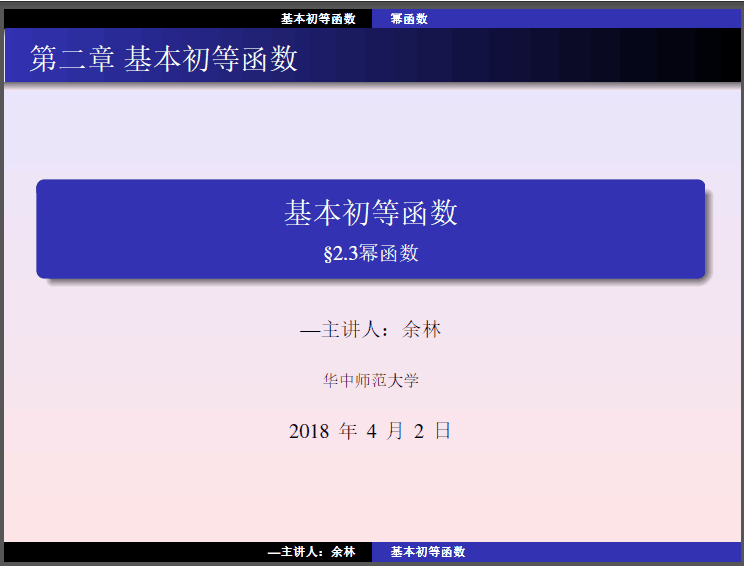
\includegraphics[scale=0.5]{1.png}
\end{center}

另一个重要的功能是\emph{语法补全},在输入各种指令时,非常容易打错,或者掉个把符号比如括号,许多代码编辑器在设定好你的编程语言后,
当你输入某些指令的前几个字符时,就会自动帮你联想可能的指令(很多时候就是你要的),这样就不容易打错,并且很多时候,插入"("等括号字符时,
会自动成对出现,避免漏掉。效果如图
\begin{center}
  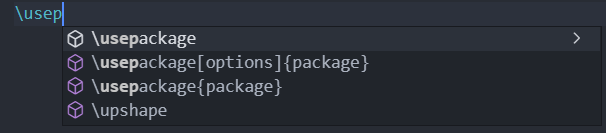
\includegraphics[scale=0.7]{2.png}
\end{center}

第三个方面是编译运行,\LaTeX{}有些代码编辑器如TeXstudio,不仅可以写代码,也提供了一键编译的按钮,如果你的编辑器没有编译的功能,就需要使用命令行编译(详见\ref{subsec:mlh}节),还有一些功能只能通过命令行使用。
这样对初学者来说上手起来就比较快。在安装\LaTeX{}时,一般会附带安装一个编辑器TeXworks,同样提供了高亮,补全,一键编译的效果,但整体比较简陋,没有
TeXstudio功能那么多,所以就会出现很多人推荐TeXstudio,导致很多人误解安装\LaTeX{}就是安装TeXstudio。

个人比较喜欢的代码编辑器是Visual Studio Code,这是微软开发的开源编辑器,具有很强的自定义性,还有各种各样实用的插件,可根据自己的需求
配置各种指令和快捷键,不过编译环境需要自己配置,可以参考这个链接:\href{https://zhuanlan.zhihu.com/p/38178015?utm_source=qq&utm_medium=social&utm_oi=1122597840500740096}{使用VSCode编写LaTeX},
推荐对\LaTeX{}有一定了解后,再更换代码编辑器提高效率。



\subsubsection{发行版}\label{subsub:fxb}


发行版指的是\LaTeX{}整个软件包的版本,\TeX{} Live,C\TeX{},MiK\TeX{}指的就是发行版,通常问安装哪个版本,指的是哪个发行版。有些模版和代码只能特定
的发行版下编译,比如本论文模版基于\TeX{} Live 2021,邓老师的旧模板基于C\TeX{},不同的发行版通常不能兼容,因此
在一般情况下\emph{请勿安装超过一个发行版!}

一个发行版主要有三个部分:各种编译器,许许多多的宏包,宏包的说明文档。宏包可以理解为指令集,提供了更多的排版指令,当你需要对应指令时,只要加载对应
的宏包就可以调用许多方便的指令。

因此,你会发现其实安装\LaTeX{},是安装这一门语言的\emph{编译环境},使得你可以在自己的电脑上编译\LaTeX{}源文件。
前面说过,如果编辑器没有没有编译的功能,就需要使用命令行编译(详见\ref{subsec:mlh}节),本质是电脑运行程序的另一种方式。
因此,\emph{安装完成后,桌面没有图标!}需要自己尝试编译一个含中文的文件,如果编译成功,才能说明安装成功,或者依照手册《install-latex-guide-zh-cn》\footnote{\url{https://gitee.com/OsbertWang/install-latex-guide-zh-cn}},这个手册非常重要,会被多次提到。




\subsection{命令行}\label{subsec:mlh}
在\ref{sub:by}节,FAQ和许多资料中都常常出现“命令行/控制台运行xx”,那么这是什么意思呢?本节解决这个问题。

\subsubsection{GUI与CLI}


我们现在的计算机操作用户界面采用图形方式显示,允许用户使用鼠标等输入设备操纵屏幕上的图标或菜单选项,这种界面称作\emph{图形用户界面(Graphical User Interface,简称GUI)}。
我们平常使用电脑主要都是在这样的界面进行的,通过鼠标打开文件,运行程序,非常方便。

\LaTeX{}是由美国计算机学家莱斯利·兰伯特(Leslie Lamport)在20世纪80年代初期开发的。在那个年代,图形界面的运用并不广泛,甚至鼠标也不普及,使用
最为广泛的用户界面是\emph{命令行界面(Command-line Interface,简称CLI)},这种界面通常不支持鼠标,用户通过键盘输入指令,计算机收到指令后,予以执行。

正是因为这样,\LaTeX{}是按照命令行界面的用户设计的,这就是为什么\emph{无论什么编译方式(包括Texstudio的一键编译),
其本质都是通过命令行运行指令调用相应的编译引擎},因此,我们需要学习一定的命令行知识。实际上,大部分的计算机语言都是类似这样,通过编译得到我们见到的软件。




\subsubsection{Windows 10系统下的命令行基本操作}\label{subsub:cz}


下面的操作均在Windows 10家庭版上完成,Mac和Linux上的操作类似。

在Windows中,命令行程序是“命令提示符”或“Windows Powershell”,可以利用菜单栏的搜索框(如图)查找。
\begin{center}
  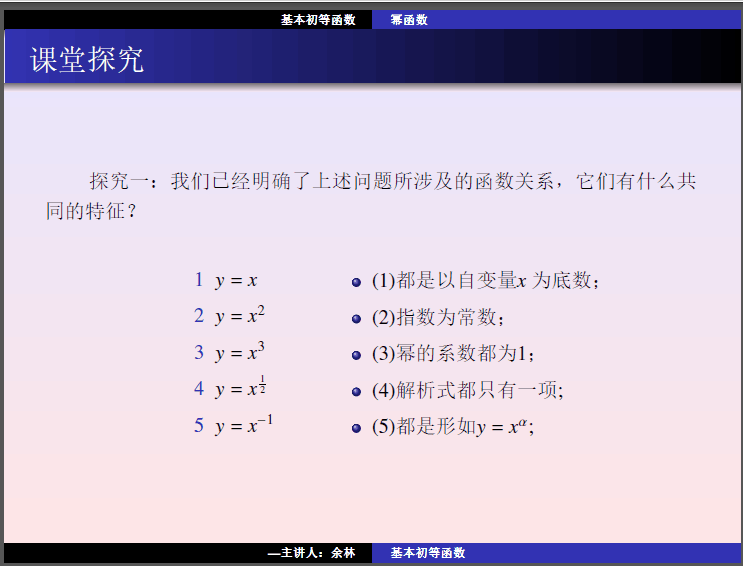
\includegraphics[scale=0.7]{3.png}
\end{center}运行时,建议右键选择“以管理员身份运行”,两个程序如图
\begin{center}
  
\includegraphics[scale=0.7]{4.png}
  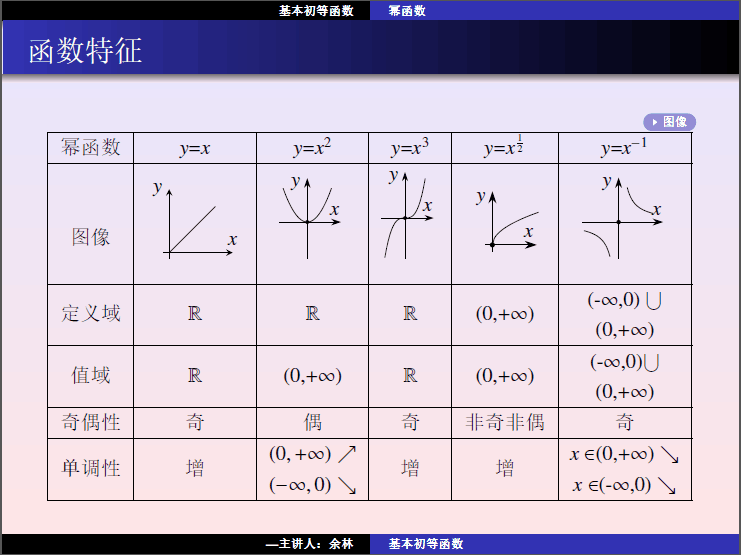
\includegraphics[scale=0.7]{5.png}
\end{center}

打开命令行窗口后(以“命令提示符为例”),会显示命令提示符(图中的红方框),由当前盘符、目录(即文件夹)和一个大于号>组成,
图中表示\emph{当前目录}为C盘WINDOWS文件夹下的system32文件夹。
\begin{center}
  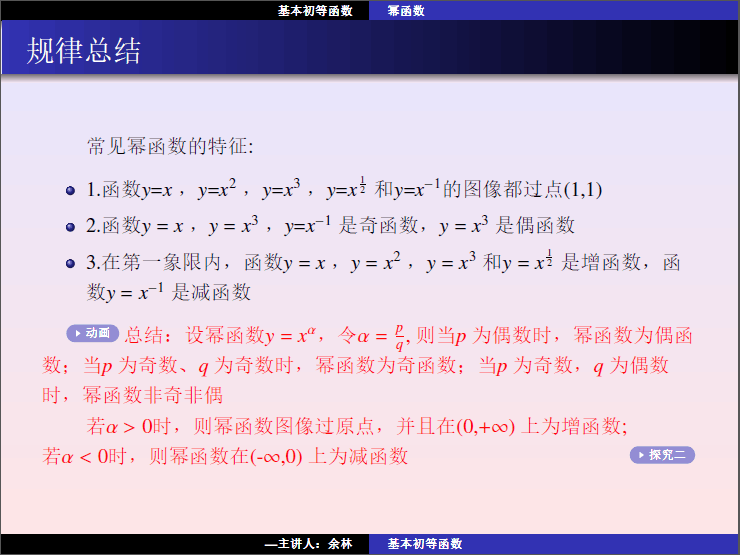
\includegraphics[scale=0.7]{6.png}
\end{center}
打开后在>的后面会有一个光标闪烁,等待输入命令,Windows命令行命令和文件名不区分大小写,输入一行
命令后按回车键执行,\emph{请注意把输入法调成英文半角,尤其是输入:和\texttt{\char92}的时候}。

下面以“用命令xelatex --shell-escape编译D盘下一个tex文件”为例进行演示

\emph{Step1:确定要编译的文件路径}

  首先找到你要编译的文件,在文件的目录的地址栏单击鼠标左键,被选中的部分就是这个文件的路径。
\begin{center}
  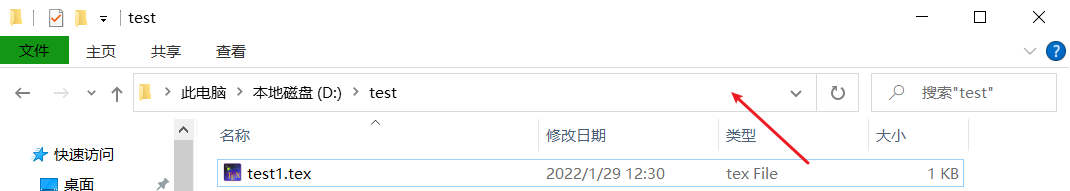
\includegraphics[scale=0.65]{7.png}
  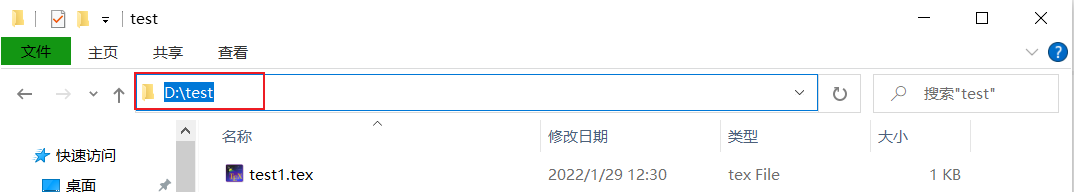
\includegraphics[scale=0.65]{8.png}
\end{center}
如图所示,源文件的存放路径是\verb"D:\test"

\emph{Step2:将命令行的当前目录切换为要编译的文件路径}

就像我们打开文件夹一样,\emph{只有命令行的当前目录为要编译的文件路径,才能进行编译},不然编译器根本找不到要编译的文件。

首先要从C盘更改为D盘,输入命令\verb"D:"后按回车键运行,会发现当前目录变成D盘。
然后输入命令\verb"cd \test"即可进入D盘下的test文件夹(目录)。
\begin{center}
  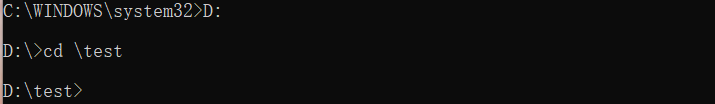
\includegraphics[scale=0.75]{9.png}
\end{center}

\emph{Step3:编译}

输入命令\verb"xelatex --shell-escape test1.tex"后按回车键开始编译,\verb"xelatex"是调用的编译器的名称;\verb"--shell-escape"是编译器的设置参数,在调用外接程序时常用;\verb"test1.tex"是要编译的文件的文件名。请注意输入法和空格!

\emph{等到再次出现命令提示符时}(如图所示),说明编译完成,此时可以回到原来的目录查看编译得到的PDF文件。
\begin{center}
  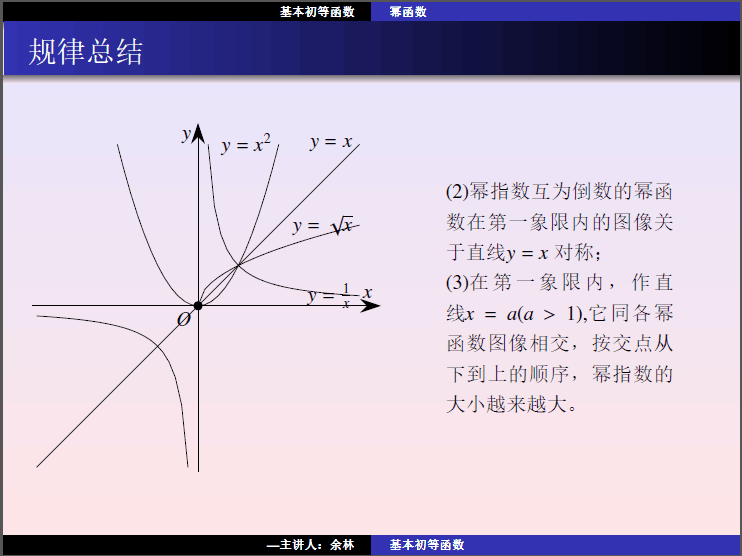
\includegraphics[scale=0.75]{10.png}
\end{center}

如果迟迟没有出现命令提示符,或者没有PDF文件,或者排版的效果非常奇怪,说明编写的代码有错误,需要进行排查。
可以阅读当前目录下生成的\verb"test1.log"日志文件,也可以直接阅读命令行窗口里的输出信息进行错误排查。由于报错
信息都是英语,需要随时准备使用翻译软件或者搜索引擎。

这个例子展示了命令行的基本用法,通过输入磁盘的字母和\verb"cd"指令进入需要运行命令的目录,再执行相应的命名,也有很多命令行
命令可以直接运行而不需要切换目录。希望大家看到“命令行下运行xx”这样的字眼时,能够不再害怕,而是尝试上手操作。



\subsubsection{Windows Terminal}


使用命令行时每次都要手动切换目录未免让人感到厌烦,Windows 10 用户可以到微软商店(Microsoft Store)下载软件“Windows Terminal”。
安装完成后重新启动电脑,你会发现右键菜单增加了选项“Open in Windows Terminal”。

\begin{center}
  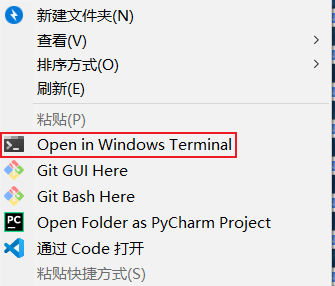
\includegraphics[scale=0.65]{11.png}
\end{center}
此时,只要在你需要进入的路径下按右键选择“Open in Windows Terminal”,弹出来的命令行窗口的当前目录就是你需要进入的路径!
但这种方式默认不是“以管理员身份运行”,因此,在一些情况下还是需要采用\ref{subsub:cz}节的方法。

\emph{总结}:本节的操作方法适用于所有需要在命令行下运行的程序,基本方法就是先用命令cd+路径或者右键菜单切换到文件的
路径,然后用程序名+(设置参数)+(文件名)的格式运行,加括号是因为有些程序不需要输入文件,或不需要设置参数。

如果你有认真读了\LaTeX{}的安装手册《install-latex-guide-zh-cn》,你会发现里面的所有操作都是基于命令行的,
通过命令行的方式进行描述使得叙述变得简单明了,碰到对应问题,在命令行下运行对应指令即可,运行指令的方法就是本节的内容。
\subsection{重要的环境变量Path}


你可能会想,能不能用命令行运行其他程序比如Word呢?然而,当你输入\verb"Word.exe"时,会得到如下的报错信息:\verb"'Word.exe'不是内部或外部命令,也不是可运行的程序或批处理文件。"

然而,你会发现,当你成功安装\LaTeX{}后,编译器的调用命令如\verb"xelatex",\verb"pdflatex"可以通过命令行在任意目录下使用;一些教程常常能看见这样的字眼“将xx添加到Path/环境变量”使人摸不着头脑,
其中的原因涉及到本节所讲的\emph{环境变量}。本节内容主要参考这个视频:\href{https://www.bilibili.com/video/BV1w741147G9?from=search&seid=9151606959931684460&spm_id_from=333.337.0.0}{『教程』什么是环境变量?}



\subsubsection{环境变量}\label{subsub:hjbl}


环境变量(environment variables)一般是指在操作系统中用来指定操作系统运行环境的一些参数,如:临时文件夹位置和系统文件夹位置等。它的主要作用,通俗来说就是\emph{指明操作系统的重要目录在哪里}。比如,环境变量 SystemRoot指明了系统目录所在的位置,
在Windows 10 的地址栏中输入\verb"%SystemRoot%"后回车,会发现跳转到C盘的Windows文件夹,这正是系统的安装目录!

显然,环境变量不止一个,打开设置,搜索“环境变量”,选择“编辑系统环境变量”,在“高级”页签右下角可以看到“环境变量”
\begin{center}
  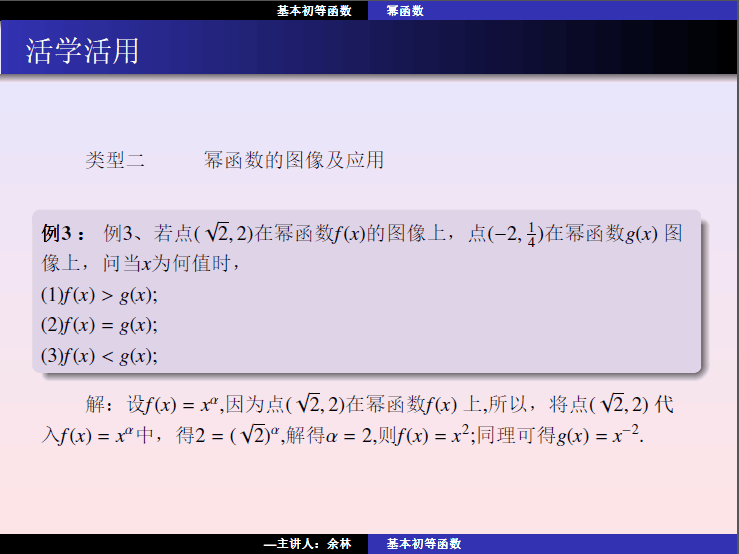
\includegraphics[scale=0.42]{12.png}
\end{center}

这样就打开了环境变量对话框,可以在这里进行编辑,会发现有\emph{用户变量}和\emph{系统变量},用户变量只针对当前登陆的用户,系统变量针对所有使用这台电脑的人,因此一般情况下只要编辑系统变量就行了。
但为了保险起见,在添加环境变量时,最好同时在系统变量和用户变量中都添加。
\begin{center}
  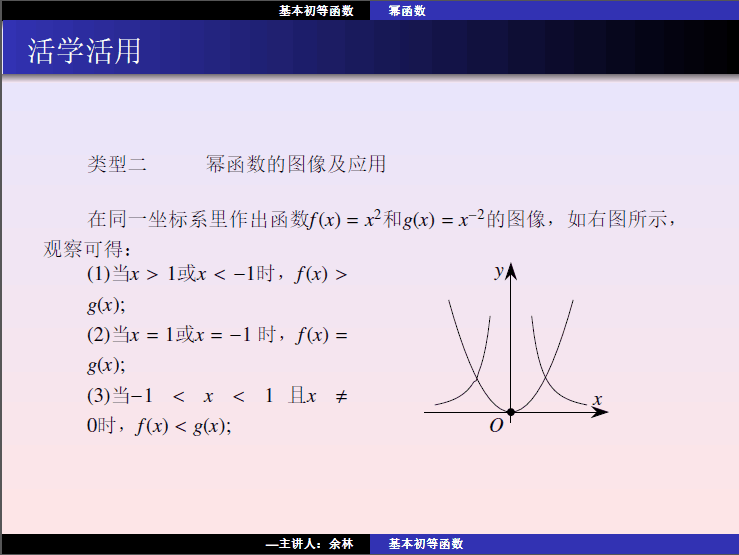
\includegraphics[scale=0.5]{13.png}
\end{center}




\subsubsection{环境变量Path}\label{subsub:pa}


Path是非常重要的环境变量,表示\emph{系统指定可执行文件的搜索路径},当在“运行”中或者命令行中输入程序的名称时,系统就会
在Path指明的目录里搜索对应的程序,找到则运行,找不到就会报错。也就是说,\emph{如果将程序A放到Path指定的目录下,这个程序就可以
随时随地通过“运行”或命令行运行!}
\begin{center}
  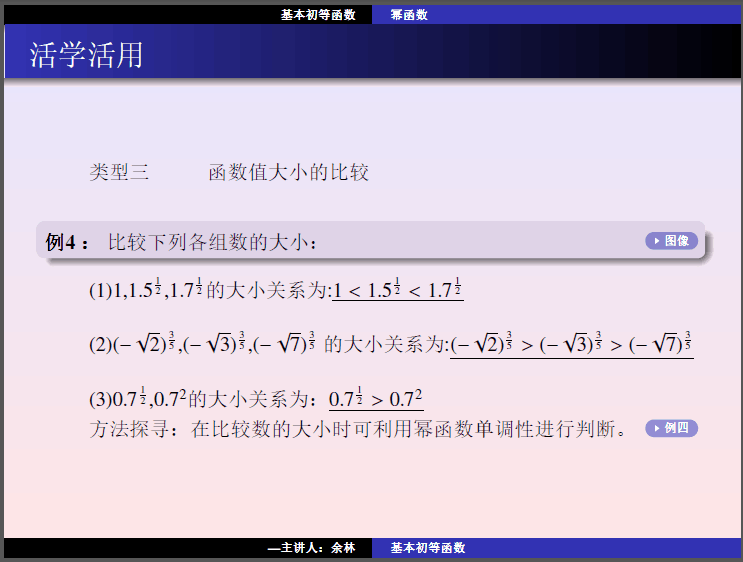
\includegraphics[scale=0.55]{14.png}
\end{center}

现在让我们看看Path的内容, 单击系统变量中Path那一行后再单击编辑,显示出来的路径就是Path指定的目录。

注意图中框起来的两个路径
\begin{enumerate}
  \item \verb"%SystemRoot%\system32"是命令提示符\verb"cmd.exe"的存放路径。
  \item \verb"E:\texlive\2021\bin\win32"是\TeX{} Live 2021的编译器和编译需要调用的程序的存放路径。安装盘符
        与安装时的选择有关,默认为C盘,我的电脑安装在E盘。
\end{enumerate}
\begin{center}
  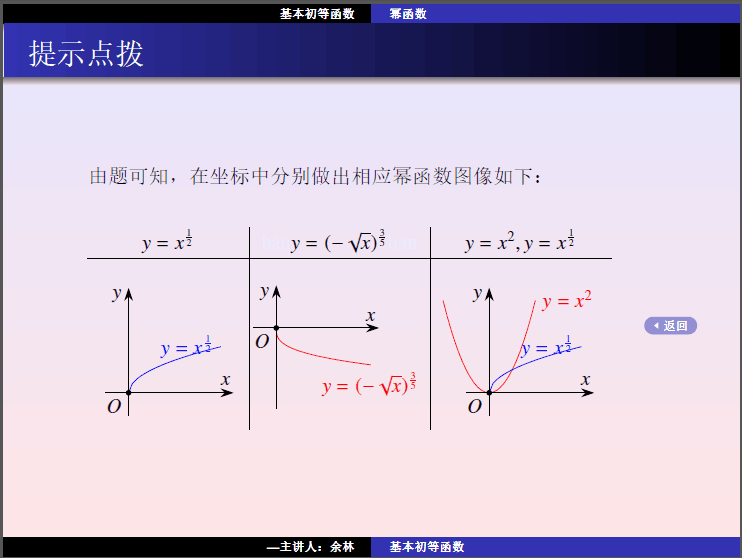
\includegraphics[scale=0.5]{15.png}
\end{center}

在Path中含有的路径下所有的可执行文件(.exe)都可以在任何地方通过“运行”或命令行直接运行,
\emph{如果发行版\TeX{} Live 2021被正确安装了,那么在电脑的系统变量Path条目中就会出现前面的路径2}。
此时,在代码编辑器点击“一键编译”或者使用第\ref{subsub:cz}节的方法在命令行下编译时,计算机才能正确的到
\TeX{} Live编译器的安装路径下找到相应的编译器运行,从而编译源代码,生成PDF文件。

也就是说,如果环境变量没有路径2,那么就无法在命令行下直接调用编译器,在编译源代码时会报错,说明\LaTeX{}安装有
问题或者根本没有安装。



\subsubsection{发行版C\TeX{}对环境变量的影响}


如果你曾经安装过C\TeX{}现在想要更换为\TeX{} Live 那么请注意,卸载C\TeX{}后,
环境变量Path可能会丢失路径\verb"%SystemRoot%\system32",请自行检查,如果丢失,则
单击“新建”,手动添加该路径到环境变量Path中。此外,如果环境变量中有mingw或jdk相关的内容,也请暂时删除,安装之后再添加到\TeX{} Live的环境变量的后面。

特别提醒,如果电脑里安装了2345好压\footnote{\textcolor{red}{警告!请务必远离所有带“2345”的软件,并且卸载时要时刻小心文字游戏!必要时借助强力卸载工具。}}这个压缩软件,也会对安装构成影响,建议卸载并更换其他压缩软件
\footnote{推荐\href{https://sourceforge.net/projects/sevenzip/}{7-Zip},\href{https://www.bandisoft.com/bandizip/}{Bandizip 6.27-6.29}或\href{http://www.winrar.com.cn/}{WinRAR}。}。

本部分详细内容见《install-latex-guide-zh-cn》的开头。



\subsubsection{添加到Path}


如果我们想让某个程序能够通过“运行”或者在命令行下直接运行,有两种方法。第一种方法是把这个程序
添加到环境变量Path指明的目录中比如提到过的system32文件夹,但这样不方便管理。
第二种方法是把这个程序所在的目录加入到环境变量Path,\emph{这就是许多教程中的“添加xx到Path”}。

在把一个程序添加到Path时,首先要找到那个程序的存放路径,方法同\ref{subsub:cz}节的Step1,然后通过\ref{subsub:hjbl}节开头的操作步骤打开环境变量,并且在Path条目里点击
“新建”,将路径粘贴进去后,先按回车键再点击确定,这样就添加完成。

有许多强力开源软件或框架\emph{只能使用命令行}操作,如Git\footnote{本手册的编写依靠它进行协作\url{https://git-scm.com/downloads}},Pandoc\footnote{强力格式转换\url{https://pandoc.org}},FFmpeg\footnote{多媒体视频处理软件,许多软件里都有\url{https://ffmpeg.org}},
Hexo\footnote{基于Git的开源博客框架\url{https://hexo.io/zh-cn/index.html}}
在安装时,如果有安装包,运行时就会自动添加相关的路径到Path,如果只有运行程序,就需要自己把程序的目录添加到Path,
这之后才能通过命令行在任意路径下使用。细心的同学可以发现在\ref{subsub:pa}节的第二张图(其实是我的电脑里的Path的截图)中有许多的软件,
比如Matlab,Pandoc,Git,Octave,FFmpeg,Python。

实际上,与\LaTeX{}相同,安装其他编程语言比如C,Python时,其实主要也是两步,
首先把编译器放到一个指定的文件夹,然后把这个文件夹的路径添加到Path中,而安装包,实际上是将这个过程包装好方便用户使用!

请特别注意,有些程序的安装包默认不把路径添加到Path,比如Visual Studio Code和Python,而是在安装时作为可选项,因此安装时
\emph{千万不要无脑点击下一步!}而是要注意勾选“添加到Path(Add to the Path)”。


\subsection{编码}\label{bm}


当你打开某些文件时,你可能发现眼前是完全无法阅读的一团乱码(比如用TeXstudio打开邓老师的旧模版),这里涉及到了编码的问题,
下面的介绍主要参考了这个视频:\href{https://www.bilibili.com/video/BV1ai4y1x7Uz?spm_id_from=333.999.0.0}{『教程』文字频频乱码,这背后是显卡的扭曲还是规则的沦丧?}



\subsubsection{编码——数字与文字的一一对应}


人类社会不仅有语言,还有各种各样的文字,承载了大量的信息,但计算机内部储存的全是二进制的0和1,如何在计算机中储存文字呢?

计算机最早诞生在美国,因此我们从英语开始。虽然美国人在做研究和说瞎话时用到的单词很多,但所有英语单词都是由26个字母组成的,
只要通过设计,让数字能够代表每一个字母,也就是建立26个字母与0和1组成的二进制代码的一一对应关系(这是一个双射!),计算机就能处理文字了。

于是,当时的科学家设计了一张表,给每一个字母(区分大小写)或符号分配一个数字,这个数字称为该字符的\emph{编码}。比如,A在这个表上对应的数字为65(在计算机里为二进制数1000001)
这张表还有一个名字,叫做\emph{美国信息交换标准代码,简称ASCII\footnote{American Standard Code for Information Interchange}}

随着时间的推移,计算机在全世界传播开来,不同的国家和地区针对自己的文字也设计了对应的编码表,比如中国设计了中文的编码表\emph{GBK},还有一个近义词叫\emph{GB 2312}.但与英文不同,汉字的
个数非常多,因此这张表很大。在中国大陆使用的Windows系统简体中文版,处理字符时默认采用GBK编码方式;中国台湾\emph{省}也有一张编码表叫做\emph{Big5}针对繁体中文。



\subsubsection{乱码问题与Unicode编码}
各个国家和地区在设计编码表时都是相互独立进行的,因此,同一段二进制代码在不同的编码表上,几乎不可能对应相同的文字。
一段文字在A国的电脑上保存时,A国电脑上的Windows系统会默认按A国的编码表把每一个字符对应的编码储存到文件里,但是,当这个文件
在B国的电脑上打开时,B国电脑上的Windows系统读取这些编码时,却会默认按照B国的编码表反推这些编码对应的字符,结果自然而然
显示出一堆乱七八糟的无意义文字,这种现象就叫做\emph{乱码}!

不同国家和地区间交换文件,不同操作系统间交换文件,都有可能出现类似的乱码情况。
\emph{乱码的本质,就是对于相同的数字编码,却用不同的编码表反推对应的字符。}这样得到的结果当然不一样,就像
破译密码时拿错了密码本。

显然,乱码问题阻碍了国际交流,一个国际组织另起炉灶,设计了一张特别大的表,叫做\emph{Unicode},这张表足够大,可以包含全人类所有的字符,这样,只要采用
这张编码表,就不会出现乱码的问题了。但在对字符分配编码的方式上,出现了许多标准,其中有一种方式是目前的主流,叫做\emph{UTF-8}。

不同的编码还给编程带来了许多麻烦,你也许听过这样的说法“安装xx时,路径不能含有中文”,“在编程时,文件夹和源代码都不能含有中文”,“系统用户名不能含有中文”。
这些问题的根源都在于简体中文版Windows系统默认采用GBK编码,而一些程序可能不支持GBK,这就产生了各种各样的问题!比如
在安装\TeX{} Live 2021时,如果系统用户名含有中文,就可能导致无法安装,解决方法还是参见《install-latex-guide-zh-cn》的1.1.3节。

然而,Mac系统却很少出现上一段的这些麻烦的问题,这是因为Mac系统默认采用UTF-8编码,兼容性好,因此Mac是非常适合编程的电脑。
一些厉害的程序员使用Mac系统编程,某些大型互联网公司甚至提供Mac作为办公电脑。



\subsubsection{\LaTeX{}中的编码问题}\label{subsub:labmwt}


许多编程语言都对源代码采用的编码方式有要求,否则无法正常编译,比如Python要求代码采用UTF-8编码方式。\LaTeX{}
比较特别,与发行版,编译引擎以及是否输入中文有关。

最早的\TeX{}系统只支持ASCII编码,但可以通过设置使得扩展ASCII编码能正常排版。在排版英文文档时,
可以直接使用pdflatex方式进行排版。

为了使得\LaTeX{}能够排版中文,Werner Lemberg开发了CJK\footnote{CJK实际上是中日韩三国语言英文单词的首字母}宏包。
由于汉字编码方式GB 2312,GBK和UTF-8都是兼容ASCII的编码,通过CJK宏包,可以把多个字符
对应到一个汉字上,支持中文的排版,在实际使用时,只要加载了CJK宏包,就可以使用pdflatex
方式进行排版。发行版CTEX支持这种方式排版中文文档,同时也是邓老师的旧模板采用的处理方式。

这种处理方法要求源文件采用GBK编码方式,存在许多问题,简单列举几个:
\begin{enumerate}
  \item CJK宏包的这种方法是一种黑客手段,没有彻底解决中文排版的问题,采用这种方式编译得到的PDF文件,其中的中文字符复制出来全是乱码!
  许多老师用C\TeX{}做的课件,里面的汉字都无法正常复制。
  \item 上面的这个问题,导致17级的同学在论文查重时,查重报告乱码!
  \item C\TeX{}目前只支持Windows系统,旧模板无法在Mac和Linux系统上使用!
  \item C\TeX{}已经停止更新,论坛已经关闭,许多遗留的bug没有修复,新的功能无法使用,网上正确且有效的资料少(英文资源几乎为零)!
\end{enumerate}
更多问题详见\href{https://zhuanlan.zhihu.com/p/45174503}{2018年,为什么不推荐使用 CTeX 套装了}。

新排版引擎\XeTeX{}和Lua\TeX{}都直接支持UTF-8编码,新的中文排版方式应运而生,孙文昌开发了xeCJK宏包,配合
xelatex方式进行中文排版,后来又出现了功能更强大的ctex宏集。\emph{新模版使用的就是这种方式,源文件采用
UTF-8编码方式,利用ctex宏集,xelatex方式进行编译}。解决了原有方式存在的许多问题。

因此,新旧模板的源代码的编码方式不同!但主流通用的代码编辑器默认都是UTF-8编码,比如TeXstudio,Visual Studio Code。
因此打开旧模板时,会直接乱码,要么采用记事本等文本编辑器,要么更改文件的编码,这就带来了许多麻烦。



\subsubsection{更改文件的编码}


通过上面的内容我们知道,当遇到乱码时或者编程语言对编码有要求时,我们都需要更改文件的编码方式。
手册《install-latex-guide-zh-cn》的第5.1.2节中提供了通过TeXstudio更改tex文件的编码方式的方法,该教程
基于英文版的TeXstudio,如果已经把界面设置为中文,请自行对照相应按键。

下面介绍使用记事本更改编码的方法:
\begin{enumerate}
  \item 找到要修改的文件,单击右键,选择“打开方式”,然后选择使用记事本打开。
  \item 菜单栏点击文件,选择另存为,在下方的编码选项中将其改为UTF-8。
  \item 最后点击保存,得到的新文件就会以UTF-8方式编码,原文件编码方式不变。
\end{enumerate}
\begin{center}
  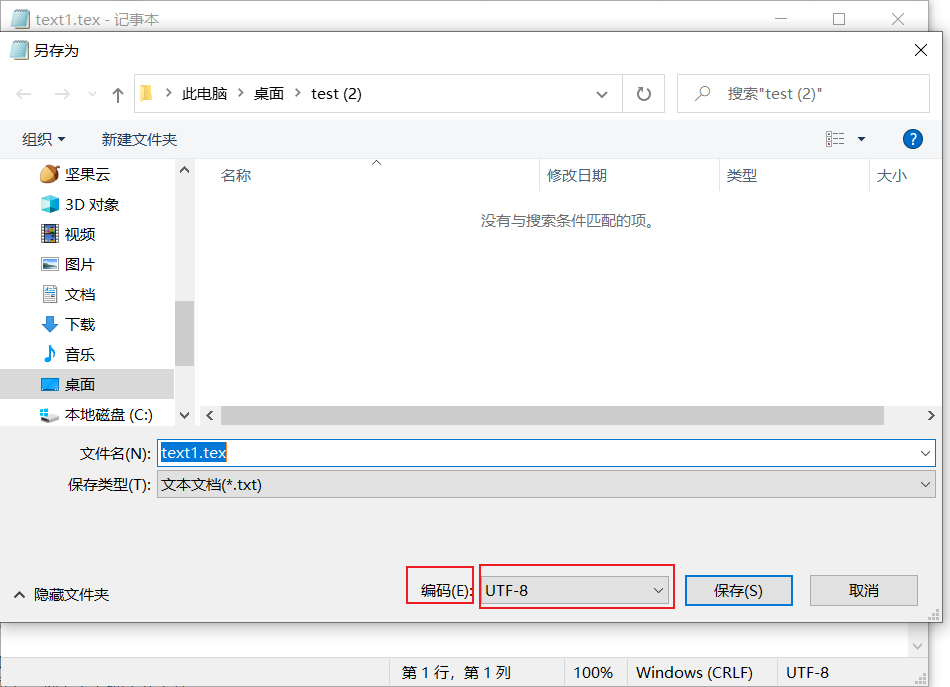
\includegraphics[scale=0.5]{16.png}
\end{center}

记事本在保存时,默认的编码为ANSI,表示当地计算机的默认编码,在中国大陆就是GBK!
因此使用记事本写代码容易因为编码而不能编译,而许多代码编辑器默认都是UTF-8编码,这
又是一个不推荐使用记事本写代码的理由。


\subsection{PDF阅读器}


PDF,全称为Portable Document Format,意为“可携带文档格式”,是由Adobe Systems用于与应用程序、操作系统、硬件无关的方式进行文件交换所发展出的文件格式。这种格式最大的优点在于,
不论在任何操作系统,手机还是电脑,最终的显示效果都是统一的,这就极大的方便了资料的传阅。\LaTeX{}代码在成功编译后,
得到的便是PDF文件,下面介绍几个PDF阅读器,用于满足两个需求,一是在写论文时随时编译查看效果,二是查看最终效果。



\subsubsection{Adobe Acrobat Reader}


Adobe Acrobat Reader是由PDF格式的设计公司Adobe推出的一款免费的PDF阅读器(请与收费的Pro版区分!)。这个阅读器的显示效果最好,且
支持PDF的所有功能(如JavaScript脚本、动画、3D对象等),\LaTeX{}的一些高级功能的效果只有使用这个阅读器才能完全显示。并且
可以查看PDF的许多属性比如使用的字体,在精细排版中会用到。

但有两个缺点,首先,安装时会强制安装在C盘,所以要记得腾空间。其次,\emph{Adobe Acrobat Reader会锁定PDF!在
Windows中重复编译时,要先关闭已经由Adobe Reader打开的PDF文档,否则PDF文件会被锁定而不能更新(同时会报错)},因此
一般在写论文途中采用其他的PDF阅读器。

下载地址:\url{https://www.adobe.com/cn/acrobat/pdf-reader.html}


\subsubsection{SumatraPDF}


SumatraPDF是一个很小的开源PDF阅读器,具有免安装版(Portable),可以放在U盘随身携带,并且打开速度非常快,适合在写作途中查看文档效果,
可以通过设置使得PDF可以反向搜索(定位到对应的代码)。当然,如果只是预览,Texwork编译后会自动弹出预览窗口。

下载地址:\url{https://www.sumatrapdfreader.org/download-free-pdf-viewer}\\或\url{https://sourceforge.net/projects/sumatrapdf-reader.mirror/}



\subsubsection{WPS}


WPS就不需要过多介绍了,与Office不同,它不强制安装在C盘。WPS包括了文字(Word),表格(Excel),演示(PPT)和PDF四个功能,安装好之后就可以直接阅读PDF文件。
顺带一提,WPS PDF可以给没有书签的PDF文档手动加书签(\emph{不需要会员!}),对于习惯使用电子书的同学会方便很多。

下载地址:\url{https://www.wps.cn/}